\documentclass[11pt,a4paper]{article}
\usepackage[utf8]{inputenc}
\usepackage{geometry}
\geometry{left=1in, right=1in, top=1in, bottom=1in}
\usepackage{booktabs}
\usepackage{hyperref}
\usepackage{amsmath}
\usepackage{parskip}
\usepackage{mathpazo}
\usepackage{graphicx}

\title{\textbf{Technical Audit Memo: Money Growth and Inflation}}
\author{}
\date{}

\begin{document}

\maketitle

\textbf{Objective:} This is an empirical setup to audit the quantity theory of money using a 160-country macro panel (1991--2024). The purpose is to decompose the broad money-inflation relationship into two distinct estimands: the long-run cross-country average and the short-run annual within-country pass-through. The core finding is that while the long-run cross-country relationship remains near one-for-one, the clean short-run within-country pass-through collapses to near-zero post-2008.

\section*{1. Data and Sample Construction}

The construction of the unbalanced panel involved merging raw World Bank WDI variables and managing severe country-specific data irregularities. This project prioritizes descriptive reliability over sample size maximization. The main sample restrictions and data checks were:

\begin{itemize}
    \item \textbf{Outlier Mitigation (The 40\% Threshold):} I trimmed the primary analytical sample to exclude countries with any year of inflation exceeding 40\%. This prevents hyperinflationary regimes (which mechanically exhibit a 1:1 money-inflation mapping) from dominating the aggregate slope and obscuring the dynamics of stable-inflation economies.
    \item \textbf{Panel Consistency ($n \ge 30$):} For long-run averages, I imposed an $n \ge 30$ threshold to ensure sufficient time-series depth for country-level aggregation.
    \item \textbf{Data Quality Note:} The raw WDI data contained a spurious $-680\%$ M2 growth rate for Sierra Leone in 2015. Investigation revealed this was a reporting/redenomination artifact (the M2/GDP level series dropped from $\sim$13,000 to $\sim$15). This observation was excluded.
\end{itemize}

\section*{2. The Empirical Contrast}

Why separate long-run versus short-run? Because the estimands capture fundamentally different economic mechanics. The long-run captures regime differences; the short-run captures annual transmission.

\textbf{Estimand A: Long-Run Country Averages}
$$ \text{average\_inflation}_i = \alpha + \beta \times \text{average\_m2\_growth}_i + \varepsilon_i $$
Countries with higher average M2 growth consistently have higher average inflation. Over 30 years, the full-sample slope is $0.952$ ($R^2=0.877$). Even in the clean sample, the slope remains strong ($0.524$). The classic Lucas (1996) result survives.

\textbf{Estimand B: Short-Run Within-Country TWFE}
$$ \text{inflation}_{it} = \gamma_i + \delta_t + \beta \times \text{m2\_growth}_{it} + \varepsilon_{it} $$
Within a country, do years with higher M2 growth see higher same-year inflation? The clean sample coefficient collapses to $0.096$.

\begin{figure}[h]
    \centering
    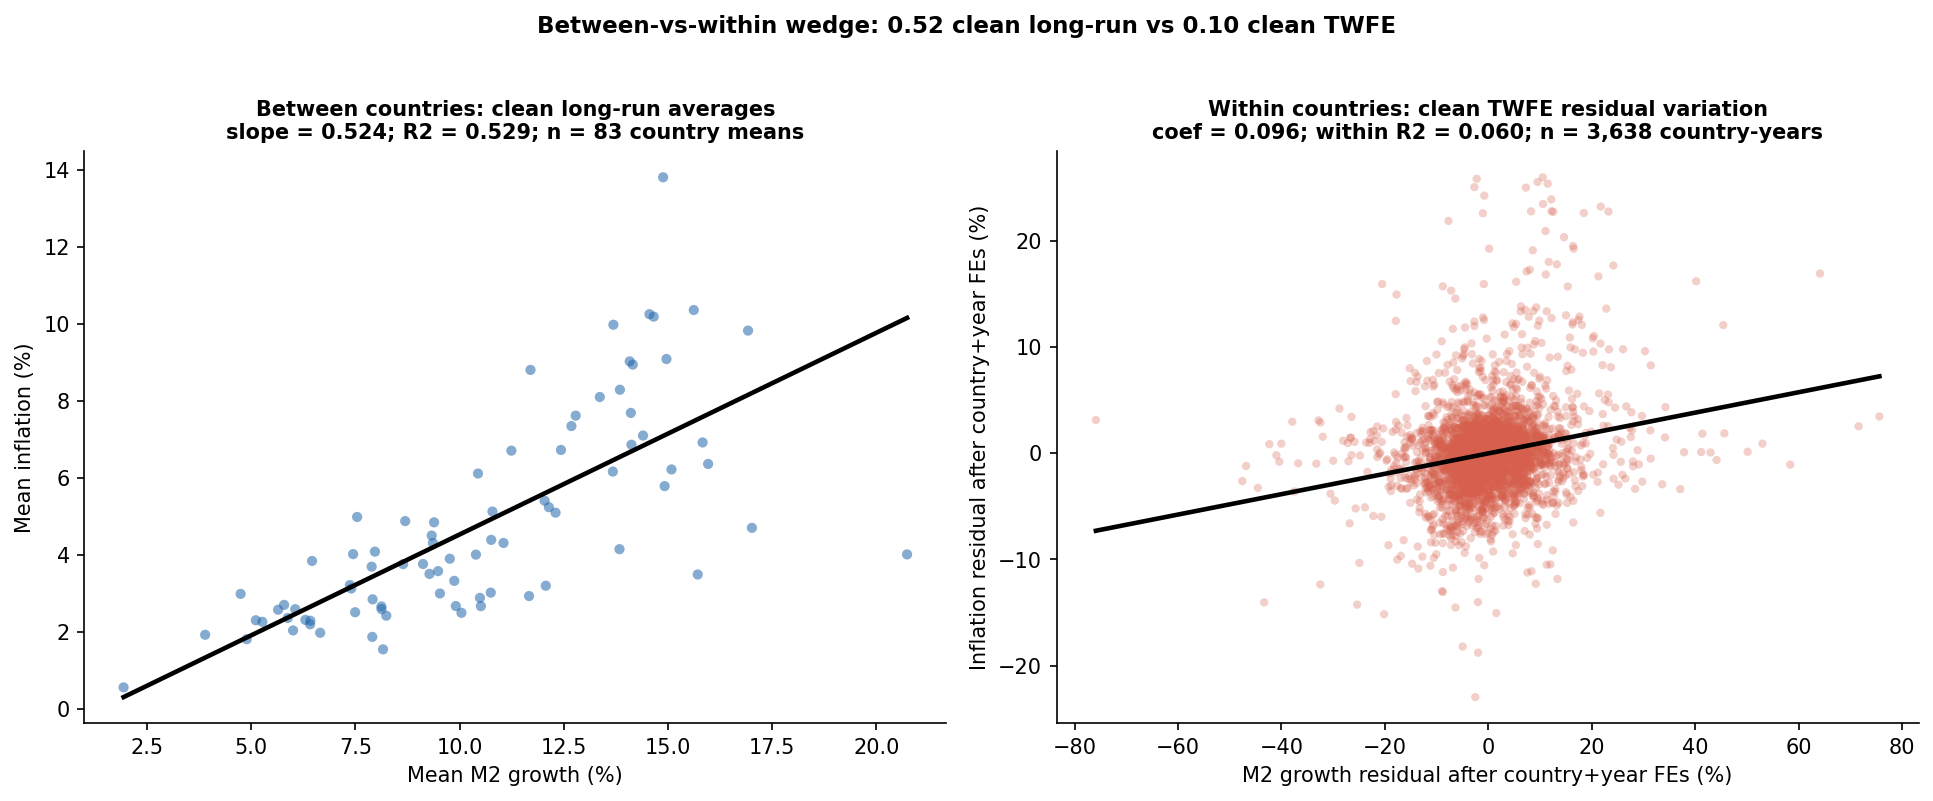
\includegraphics[width=0.85\textwidth]{04_current_results/figures/between_within_decomposition.png}
\end{figure}

Why the pre/post-2008 split? The 2008 financial crisis fundamentally altered monetary transmission (e.g., QE, excess reserves). Splitting the TWFE exposes the structural shift:
\begin{itemize}
    \item \textbf{1991--2007:} Slope is $0.113$ ($p<0.001$).
    \item \textbf{2008--2019:} Slope is $-0.006$ and statistically insignificant ($p=0.711$).
    \item \textbf{2020--2024:} Slope is $-0.014$ and statistically insignificant ($p=0.655$).
\end{itemize}
Short-run pass-through drops to near-zero in both clean-sample post-2008 cuts.

\begin{figure}[h]
    \centering
    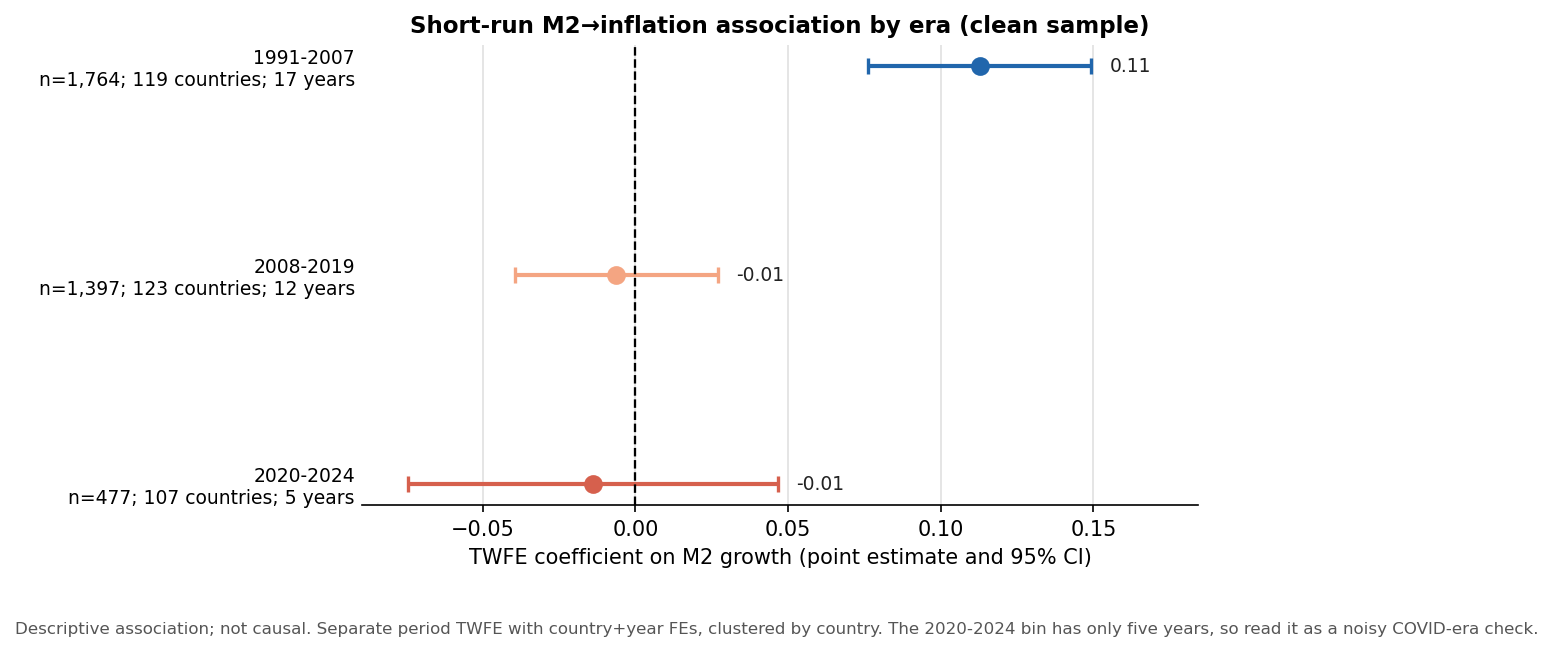
\includegraphics[width=0.7\textwidth]{04_current_results/figures/pre_post_2008_coef_plot.png}
\end{figure}

\section*{3. Key Limitations \& Methodological Restraint}

This project is strictly a descriptive empirical audit. I intentionally avoided causal overclaiming:

\begin{itemize}
    \item \textbf{Instrumental Variables (IV) Rejected:} I explored Local Projections IV (LP-IV) using external lending rates and lagged M2 as instruments. The primary instrument yielded a first-stage F-statistic of 5.96. The secondary instrument was mechanically strong ($F=16.29$) but the exclusion restriction was not credible. Therefore, I explicitly chose not to run headline IV. A weak identification strategy damages credibility more than admitting the limits of OLS. The IV results are retained solely as a directional appendix.
    \item \textbf{Inflation Targeting (IT):} I ran an event study on IT adoption. While IT adopters show a sharp post-adoption drop in the money-inflation slope (from 0.279 to 0.038 in the clean sample), IT adoption is endogenous. This is associational heterogeneity, not a causal treatment effect.
    \item \textbf{COVID as Stress Test, not Design:} The 2020--2023 COVID episode shows a positive cross-country money-inflation slope ($0.494$), but it cannot isolate broad money from fiscal transfers or supply shocks. It remains descriptive.
\end{itemize}

\end{document}
